\problemname{Find the k-th Occurrence}

In our Tower of Hanoi puzzle, we will use a string to represent the location of each disc.
The discs will be numbered $1, 2, ..., n$ where, $1 \leq n \leq 9$.
The larger the number, the larger the disc.
For each of the three pillars, we will list the discs starting from the bottom e.g. $321$.
We will use the \texttt{|} character to signify the end of the disc sequence for a particular pillar.
Here are a few examples:

\begin{figure}[h]
    \centering
    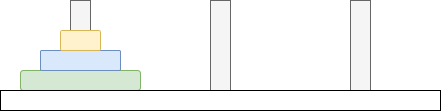
\includegraphics[width=0.5\textwidth]{1}
    \caption{\texttt{321|||}}
\end{figure}

\begin{figure}[h]
    \centering
    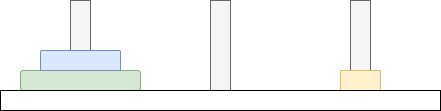
\includegraphics[width=0.5\textwidth]{2}
    \caption{\texttt{32||1|}}
\end{figure}

\begin{figure}[h]
    \centering
    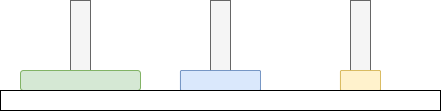
\includegraphics[width=0.5\textwidth]{3}
    \caption{\texttt{3|2|1|}}
\end{figure}

We are going to need a function
that finds the location of the $1st$, $2nd$ or $3rd$ \texttt{|} character within that string
so that we know from where to remove or add characters as we move the discs about.
More generally, we would like to find the index of the $k$-th occurrence of an element
within a sequence.
So that is your task in this first part. Write the function

\texttt{find\_index\_of\_kth\_occurrence(sequence, element\_to\_find, occurrence)}\\
that finds the position of a given occurrence of an element within a sequence.
See below for the exact specifications.

\textbf{Note that we are testing your code differently in this task,
please only submit your function definitions, without any code outside the functions!}
The main python file, which handles input and output, is already provided.
You can download and place the main file in the same directory as your python file.
You can then run the main python file we provide to try out the samples.

\section*{Input}
The function receives three parameters,
a string $s$, an element $e$ and an integer $k$.
In the tests, $s$ will be a string with $1 \le |s| \le 20$,
$e$ will be a single character, that is, a string of length $|e| = 1$,
and $k$ will be restricted to $1 \le k \le 20$.
You may assume all characters in the input are printable ASCII characters.

It is good if your function also works for other types of sequences and elements,
or for input outside these specifications,
but you do not need to worry about that.

In the samples below,
the first line of the input contains the string $s$,
the second line contains the character $e$
and the third line contains $k$.

\section*{Output}
The function should return one integer $i$,
the position of $k$-th occurrence of the element $e$ within the sequence $s$
or $-1$ if there are less than $k$ occurences of $e$ within $s$.

In the samples below,
the first and only line of the output contains the integer $i$.
